% Template for a Computer Science Tripos Part II project dissertation
\documentclass[12pt,a4paper,twoside,openright]{report}
\usepackage[pdfborder={0 0 0}]{hyperref} % turns references into hyperlinks
\usepackage[margin=25mm]{geometry} % adjusts page layout
\usepackage{graphicx} % allows inclusion of PDF, PNG and JPG images
\usepackage{verbatim}
\usepackage{docmute} % only needed to allow inclusion of proposal.tex\newcommand{\code}{\texttt}
\usepackage{amsmath}
\usepackage{color}
\usepackage{siunitx}
\usepackage{gensymb}
\usepackage{tikz}
\usepackage{pgfgantt}
\usepackage{lscape}

\definecolor{dkgreen}{rgb}{0,0.6,0}
\definecolor{gray}{rgb}{0.5,0.5,0.5}
\definecolor{mauve}{rgb}{0.58,0,0.82}

\raggedbottom % try to avoid widows and orphans
\sloppy
\clubpenalty1000%
\widowpenalty1000%
\renewcommand{\baselinestretch}{1.1} % adjust line spacing to make
\newcommand{\code}{\texttt}
% more readable
\begin{document}
\bibliographystyle{plain}
%%%%%%%%%%%%%%%%%%%%%%%%%%%%%%%%%%%%%%%%%%%%%%%%%%%%%%%%%%%%%%%%%%%%%%%%
% Title
\pagestyle{empty}
\rightline{\LARGE \textbf{Jeffrey Song}}
\vspace*{60mm}
\begin{center}
\Huge
\textbf{Building a Physics Engine From Scratch} \\[5mm]
Computer Science Tripos - Part II \\[5mm]
Robinson College \\[5mm]
\today % today's date
\end{center}
%%%%%%%%%%%%%%%%%%%%%%%%%%%%%%%%%%%%%%%%%%%%%%%%%%%%%%%%%%%%%%%%%%%%%%%%%%%%%%
% Proforma, table of contents and list of figures

\newpage
\section*{Declaration of originality}
I, Jeffrey Song of Robinson College, being a candidate for Part II of the Computer Science Tripos, hereby declare that this dissertation and the work described in it are my own work, unaided except as may be specified below, and that the dissertation does not contain material that has already been used to any substantial extent for a comparable purpose. In preparation of this dissertation I did not use text from AI-assisted platforms generating natural language answers to user queries, including but not limited to ChatGPT. I am content for my dissertation to be made available to the students and staff of the University.
\bigskip
\leftline{Signed Jeffrey Song}
\medskip
\leftline{Date \today}
% \section*{Acknowledgements}

\pagestyle{plain}
\chapter*{Proforma}
{\large
\begin{tabular}{ll}
Candidate Number: & \bf 2419E \\
College: & \bf Robinson College \\
Project Title: & \bf Building a Physics Engine From Scratch \\
Examination: & \bf Computer Science Tripos -- Part II, May 2024 \\
Word Count: & \bf TBA\footnotemark[1] \\
Code Line Count: & \bf TBA\footnotemark[2] \\
Project Originator: & The candidate \\
Project Supervisor: & Joseph March \\
\end{tabular}
}
\footnotetext[1]{This word count was computed
by \texttt{detex diss.tex | tr -cd '0-9A-Za-z $\tt\backslash$n' | wc -w}
}
\footnotetext[2]{This line count was computed
by TBA
}
\stepcounter{footnote}

\section*{Original Aims of the Project}

This project takes interest in building a simplified but functional physics engine, primarily focusing on implementing rigid body simulation. With its core being a software engineering challenge, it also heavily involves some computational geometry and physics formulation. The physics engine in the end is expected to be able to simulate the movement of rigid bodies in 3D space, including their position, rotation and collision. These interactions should then be tested with simple experiments against more popular and available physics engines. As extensions, evaluation of its performance and other more in-depth mechanics like soft body simulation can be built on top.

\section*{Work Completed}

This project has completed all success criteria. A physics engine is built to simulate rigid body dynamics, with collision handling in place. Then, I used a rendering software Blender to test out its APIs, and successfully generated examples of simple working experiments using rigid body simulation. Finally, I collected a few public physics engines and compared mine with them on some simple physical experiments to compare the performance. The result showed that my physics engine was able to generate comparable results.

\section*{Special Difficulties}

None.

\newpage

\tableofcontents
\newpage

%%%%%%%%%%%%%%%%%%%%%%%%%%%%%%%%%%%%%%%%%%%%%%%%%%%%%%%%%%%%%%%%%%%%%%%
% now for the chapters
\pagestyle{headings}

\chapter{Introduction}

\section{Background}

Physics Engine attempts to simulate real life physical properties through well-known physics laws. Starting as a branch of computer graphics, they quickly became commonly used in video games, since many games try to resemble what we already have in the real world. In general, this is done with a physics engine, encapsulating most physics simulation modules. They are then incorporated into the game engine itself, allowing scripts to easily control the movement and settings of important game objects. The most popular game engine for example, Unity\cite{unity}, has its own implementation of physics engine.

It then becomes significantly easier for game developers to simulate realistic effects. For example, to create "Flappy Bird\cite{flappybird}" in unity, the bird could be attached with a rigid body physics component, which could then modify the movement of the bird according to gravity with response to player controls. The underlying physics engine sees the rigid body, and attempts to modify its position and rotation according to physics law. This engine integration has become an important tool of game development.

\section{Motivation}

Nowadays, many developers choose to rely on whatever comes as built-in for their choice of engine. Unity, for example, has an integration of the NVIDIA PhysX engine, which is provided under a freeware license. Other popular choices include many open-source physics engines, for example SOFA\cite{sofa}. These ready-made tools are well-polished by big communities and have in-depth support for most functionalities the developers want. However, it's also not rare to see people create their own custom physics engine, as this allows for greater customization possibilities, and some ideas might eventually get contributed to the open-source community. I also take interest in setting up a physics engine from scratch of my own, additionally granting me learning experiences for underlying physics mechanics and software engineering problem solving.

While physics engine consists of many possible components that are considered on-going research problems, a main building block of it - Rigid body dynamics\cite{rigidbodydynamics}, is more widely used and accepted, with many well-established implementations and experiments. Rigid body dynamics studies systems of interconnected bodies which do not deform under applied forces. Relative position is preserved inside each rigid body, making it easy to calculate positions relative to the world. Despite the rigid assumptions imposed on the physical objects, rigid body simulation gives rise to quick use of well-known physical laws and common experiments, which would set the core fundamentals for this project.

\section{Previous related work}

There has been continuous efforts on physics simulation particularly in game industries. The development is marked by several big physics engine projects, with some of them still being frequently used to this day. Some milestones in this industry include:

\begin{itemize}
\item Havok Physics engine\cite{havoks}, as one of the pioneering physics engine in the early 2000s. Developed by the company Havok, related SDK saw stable release and development still to this day.
\item Open Dynamics Engine (ODE)\cite{smith2005open} provides a widely used open-source framework for rigid body dynamics. As another early 2000s project, it has a great impact on subsequent related researches.
\item Bullet\cite{bullet}, provides a free and open-source software for soft and rigid body dynamics, currently hosted on github\cite{bulletgithub}.
\item PhysX\cite{physx}, with full support from NVIDIA, acquired much popularity with its wide range of simulation features in real-time uses. Some of the more complicated features like fluid simulation were made easy to be use, attracting many developers.
\item Unity and Unreal Engine\cite{sanders2016introduction} are modern game developing engines which have physics engines components incorporated along with other development utilities. Unity uses a version of PhysX while Unreal uses its in-house physics engine. As  complete development tools these game engines are becoming widely used for many purposes.
\end{itemize}

Other new physics engines are being actively developed and published, for example brax\cite{freeman2021brax}, Jade\cite{yang2023jade}, and so on.

Meanwhile, there are also many recent researches concerning some of the physics simulation mechanics both in theoretical level and in application level.

Many theoretical explorations focus on improvements on efficiency and precision. Rigid body simulation\cite{singh2022efficient}, soft body simulation\cite{li2022contact}, and fluid simulation\cite{obiols2020cfdnet}, \cite{klower2022fluid}, \cite{vinuesa2022enhancing} have all been receiving new methods to compute efficiently and accurately.

Application level researches demonstrate several science or real life applications assisted by relevant physics simulation. Examples include \cite{wang2020spring}, \cite{nampoothiri2023slip} and \cite{he2021simulation}.

\section{Structure of the dissertation}

The following Chapter \ref{chap2} presents theoretical background maths for implementing rigid body simulation. Chapter \ref{chap3} highlights some of the software engineering challenges along with some extra relevant algorithms for tackling a few specific problems. In Chapter \ref{chap4}, some evaluations are conducted for the physics engine using simple experiments and comparisons. Finally, Chapter \ref{chap5} discusses my personal lessons and success, while giving some ideas for potential future work.

\chapter{Preparation}\label{chap2}

\section{Starting point}

\subsubsection{Knowledge}

Relevant knowledge came from NST Maths in IA, Introduction to Graphics in IA, and Complexity Theory in IB, despite them being only helpful in providing concepts and basic ideas for manipulating computational geometry. I had previously briefly touched on computational geometry related algorithms in coding practicing sites like leetcode prior to the project.

\subsubsection{Reference material}

I did not read any of the tutorials and guides prior to the project, but I knew they existed in a somewhat plentiful quantity, which lent me some confidence. After starting with the project, I read many of them during the early stages of implementation, including \cite{tutorial1}, \cite{tutorial2} and \cite{tutorialyt}.

\subsubsection{Codebase and libraries}

I decided to use C++ as the main programming language for the project, which Programming in C and C++ in IB had partially covered, plus me having some experience with it from coding tutorials online. However, I do not have profound experience with building projects using C++, so I do have to learn the repository structure alongside with deploying automated build systems for C++.

As for the libraries, I had no experience with any of the relevant rendering libraries, so I had to learn from scratch on using Blender\cite{blender}. Its documentation page with scripting\cite{blenderdoc} helps a lot. Besides Blender, several third-party libraries provided support for utitilies like testing and plotting. I also tried importing some other libraries during development but later removed them due to them not being helpful.

Table \ref{tplbl} lists out all third-party software I have used in the current project/

\begin{table}[h]\label{tplbl}
    \centering
    \makebox[\linewidth]{
    \begin{tabular}{|c|c|c|}
    \hline 
    \textbf{Third-party software} & \textbf{Usage} & \textbf{License} \\
    \hline 
    numpy & Efficient arrays for data management & BSD License \\
    matplotlib & Plotting diagrams for data & PSF License \\
    CMake & C++ Build system & BSD License \\
    Makefile & Build automation tool & - \\
    scipy & Conversion of rotations & BSD License \\
    Blender & 3D modeling and animation & GPL License \\
    \hline
    \end{tabular}
    }
    \caption{List of Third-Party Software Used}
    \label{tab:third_party_software}
\end{table}

\subsubsection{Development tools}

I used Visual Studio Code on my laptop (11th Gen Intel(R) Core(TM) i7-11800H @ 2.30GHz CPU, 16.0 GB RAM, NVIDIA GeForce RTX 3050 Laptop GPU) for engine implementation. Some plots and tests were done with Google Colab and Kaggle Notebook. Platforms including GitHub and Google Drive allowed for backups and simple version control for the project. For the writeup of this dissertation, Overleaf helped with \LaTeX compilation and file management.

\section{Structure of the engine}

Physics engine here in my project specifically refers to Rigid body simulation, as it is the main component and the building block of any large-scale complete game engine. Other possible compoents are considered extensions. The main working loop of the engine could be described by a simple feedback loop framework by figure \ref{looplbl}.
\begin{figure}\label{looplbl}
    \centering
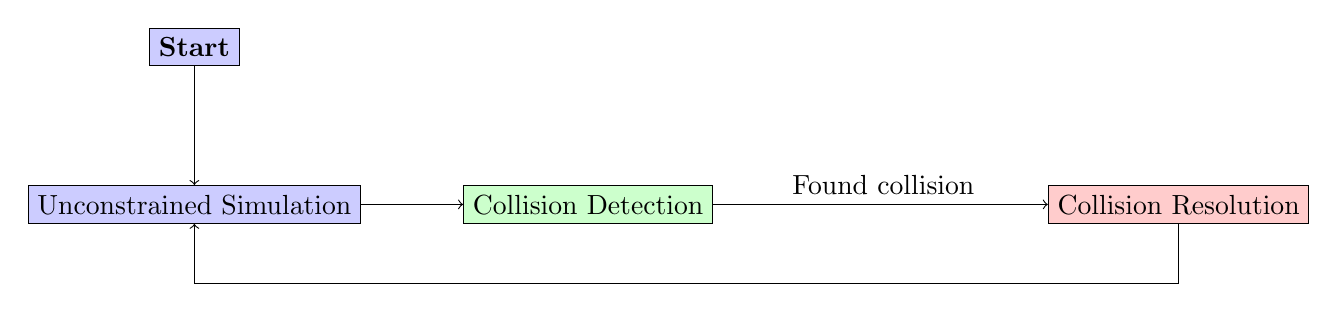
\begin{tikzpicture}
    \node [draw, fill=blue!20] at (0,0) (a) {\textbf{Start}};
    \node [draw, fill=blue!20] at (0,-2) (b) {Unconstrained Simulation};
    \node [draw, fill=green!20] at (5,-2) (c) {Collision Detection};
    \node [draw, fill=red!20] at (12.5,-2) (d) {Collision Resolution};
    \node[draw=none] at (8.75, -1.75) (e) {Found collision};
    \node[draw=none] at (8.75, -3) (f) {};
    \node[draw=none] at (9.15, -3) (g) {};
    \path [draw, ->] (a) -- (b);
    \path [draw, ->] (b) -- (c);
    \path [draw, ->] (c) -- (d);
    \path [draw, -] (d) |- (f);
    \path [draw, ->] (g) -| (b);
\end{tikzpicture}
\caption{Core Feedback Loop}
\end{figure}

After the initial setup of the objects as rigid bodies, the engine begins a main feedback loop. Each iteration of the loop attempts to advance the simulation by a small time frame, and at the end of each time frame, the position and rotation data could be updated, and then serialized and exported to the rendering software, currently Blender.

In each iteration of the loop, all rigid bodies are assumed to start in a nonpenetration state, that is, no pairs of rigid bodies intersect with each other. But touching on some faces are allowed. Then, we perform the unconstrained simulation for a small timeframe $dt$. During this simulation it is assumed that no collisions happened. Finally, collision detection and resolution are performed, correcting mistakes from the unconstrained simulation. Some more details of these steps are described below.

\subsection{Rigid body modelling}

In general, the goal of unconstrained simulation is to first track the status of all rigid bodies as reasonable mathematical data structure, and then update them assuming no collisions ever happen.

The state of a rigid body entails the location $x$, rotation $R$, linear momentum $p$, and angular momentum $L$, relative to the centre of the entire simulation space. The location and rotation in particular encapsulates where to place them in the world, and need to be exported for rendering at the end of each iteration. The entire state can be expressed as a tuple of these information, say $S = (x, R, p, L)$, and it gives the main moving characteristics of the rigid body. This state can be viewed as a function of time $t$. The derivative of the state with respect to time, $\frac{d}{dt}S$, can then be derived using variables from $S$, which would be used when advancing by the small time frame $dt \approx \frac{1}{30}s$ for example in 30 fps rendering.

\begin{equation}
\frac{d}{dt}S = (\frac{d}{dt}x, \frac{d}{dt}R, \frac{d}{dt}p, \frac{d}{dt}L)
\end{equation}

Each element of the state needs to be defined then differentiated separately.

\subsubsection{Location $x$} 

A 3-element vector containing the $x$ $y$ $z$ coordinates of the center of the rigid body relative to the world center. The center of a rigid body is the center of mass, which is defined as

\begin{equation}
x=\frac{\sum{m_i}{x_i}}{M}\label{eq:3}
\end{equation}

if we consider the body is made up of many small particles, the $i$-th one at position $x_i$ in world space while having mass $m_i$. $M$ is the total mass of the body

\begin{equation}
M=\sum{m_i}
\end{equation}

Here $x_i$ are vectors and masses are scalars, so the center of mass is a vector of the center of mass coordinates. For simplicity think of it as the geometric center of the body, and think of the density to be uniform across the body.

Differentiating $x$ gives the linear velocity $v$.

\begin{equation}
v = \frac{d}{dt}x
\end{equation}

\subsubsection{Rotation $R$} 

A $3\times 3$ matrix describing how the rigid body has rotated around its center. For any particle on the body, consider $r_i$ to be its body space location, i.e. the coordinates if the body is placed upright, with its center of mass located at the origin $(0, 0, 0)$. Then, the world space location of the particle $x_i$ can be computed with the help of the rotation matrix, then translated using the location of the center of mass

\begin{equation}
x_i = R\times r_i + x\label{eq:1}
\end{equation}

$R$ is a rotation matrix, which comes with many properties, for example if

\begin{equation}
    R = \begin{pmatrix}
        R_{xx} & R_{xy} & R_{xz} \\
        R_{yx} & R_{yy} & R_{yz} \\
        R_{zx} & R_{zy} & R_{zz}
    \end{pmatrix}
\end{equation}

then multiplying R by an axis-aligned unit vector, say $(1, 0, 0)$, gives the result of rotating the corresponding axis

\begin{equation}
R \times\begin{pmatrix}
    1 \\
    0 \\
    0
    \end{pmatrix}
    =
    \begin{pmatrix}
    R_{xx} \\
    R_{yx} \\
    R_{zx}
    \end{pmatrix}
\end{equation}

Angular velocity $\omega$ is used to describe the speed of rotation. Slightly counterintuitively, $\omega$ is a vector, where its direction gives the rotating axis and its magnitude gives the speed.

Clearly differentiating the rotation matrix $R$ does not give the angular velocity vector $\omega$. Instead, with some careful analysis, we would obtain % APPENDIX?

\begin{equation}
\frac{d}{dt}R = \omega ^* \times R
\end{equation}

where $v^*$ is the star operation that transforms vector $v=(x, y, z)$ to a matrix:

\begin{equation}
    v^* = \begin{pmatrix}
        0 & -z & y \\
        z & 0 & -x \\
        -y & x & 0
    \end{pmatrix}
\end{equation}

Note a useful property of this operation

\begin{equation}
    a^* b = a \times b\label{eq:2}
\end{equation}

\subsubsection{Linear momentum $p$} 

The linear momentum $p$ is defined as sum of products of mass and velocity of all particles comprising the body

\begin{equation}
    p = \sum m_i v_i
\end{equation}

making $p$ a vector.

Velocity of a particle $v_i$ is the derivative of its world space location $x_i$

\begin{align*}
    v_i &= \frac{d}{dt}x_i \\
        &= \frac{d}{dt}(R r_i + x) && \text{(by equation \eqref{eq:1})} \\
        &= \omega^* R r_i + v \\
        &= \omega \times (R r_i) + v && \text{(by equation \eqref{eq:2})} \\
        &= \omega \times (R r_i + x - x) + v \\
        &= \omega \times (x_i - x) + v
\end{align*}

Now to derive $p$

\begin{align*} 
    p &= \sum m_i v_i \\
      &= \sum m_i (\omega \times (x_i - x) + v) \\
      &= \sum m_i v + \omega \times \sum m_i (x_i - x) \\
      &= \sum m_i v + \omega \times (\sum m_i x_i - M x) \\
      &= \sum m_i v && \text{(by equation \eqref{eq:3})} \\
      &= (\sum m_i) v \\
      &= M v
\end{align*} 

Differentiating $p$ gives the total force $F$ acting on the body

\begin{equation}
\frac{d}{dt} p = F
\end{equation}

The force can be imagined as the sum of the forces on every individual particle of the body

\begin{equation}
F = \sum F_i
\end{equation}

\subsubsection{Angular momentum $L$} 

Angular momentum $L$ is a vector defined by

\begin{equation}
L = I \omega
\end{equation}

where $I$ is a $3\times 3$ matrix known as inertia.

\begin{equation}
I = R I_{body} R^T
\end{equation}

where $I_{body}$ is a constant matrix describing the shape of the rigid body, calculated in body space
    
\begin{equation}
I_{body} = \sum m_i((r_i^T r_i)\textbf{1} - r_i r_i^T)
\end{equation}

where $\textbf{1}$ is the identity matrix.

Torque $\tau_i$ as a vector describes how the body would rotate if individual force $F_i$ is applied to each particle. Total torque $\tau$ is the sum of individual torque.

\begin{equation}
\tau_i = (x_i - x) \times F_i
\end{equation}

\begin{equation}
\tau = \sum \tau_i
\end{equation}

Differentiating $L$ gives the total torque $\tau$, similar to how differentiating $p$ gives the total force $F$.

\begin{equation}
\frac{d}{dt} L = \tau
\end{equation}

\subsection{Collision detection and resolution}

If at the end of the timeframe two rigid bodies end up clipping into each other, then there must have been a collision during the timeframe, meaning the states need to be corrected. This is done by first scanning for collision detection, and if detected, calculate relevant contact information, such as when and where two objects collide. Then the information will be used for collision resolution, where the velocity needs to be corrected before resuming the simulation.

\subsubsection{Collision detection}

Finding separating plane is a popular method for detecting collisions among convex polyhedrons. Concave objects are trickier to deal with, and luckily most concave objects are good enough when represented by a bounding convex object in practice. In rare cases convex decomposition is required, which is far more complicated and computationally intensive, with the current popular choice being V-HACD\cite{mamou2016volumetric}, and its complexity should be outside the scope of this project.

Consider two convex polyhedrons A and B. They are considered to be collided if any point in A is also in B. It is actually easier to detect if the pair has not collided, in which case no part of the two objects intersect. Note that having some parts touched between them does not count as collision, so as to avoid repeatedly resolving collision when two touching objects happen to move at the same speed. Using the convex property, there must be a separating plane that separates the space into either only containing A or only containing B.

Furthermore, it is sufficient to only consider two cases. When both cases fail, it can deducted that no separating planes exist.

\begin{itemize}
\item Face-vertex collision. Consider the separating plane to be one of the faces of the original objects.
\item Edge-edge collision. Consider the separating plane to be between one edge of A and one edge of B, with its normal equal to the cross product of these two edges. 
\end{itemize}

Both cases can be checked by brute force over faces or edges of the two objects.

In the case a collision does happen, find the exact moment the contact takes place, and record the normal of the separating plane at that moment, say $n$, as well as the points on the two bodies that contact. Next, hand the information over to collision resolution.

\subsubsection{Collision resolution}

Only the velocities at direction $n$ are altered after the collision takes place, so the first thing is to obtain component of the relative velocity in the $n$ direction using dot product.

\begin{equation}
v_{AB} = n \cdot (v_B - v_A)
\end{equation}

where $v_{AB}$ measures the relative velocity as a scalar, while $v_A$ and $V_B$ are the velocity of the contacting points on object A and B respectively at the moment of collision.

The law of collisions states

\begin{equation}
v_{AB}' = -\epsilon v_{AB}
\end{equation}

where $v_{AB}'$ is the same quantity after the collision happens, and $\epsilon$ is the coefficient of resititution.

This coefficient $\epsilon$ satisfies $0 \leq \epsilon \leq 1$. At $\epsilon = 0$, two bodies will move together after collision, known as resting contact. At $\epsilon = 1$, two bodies perfectly bounce backwards. In practice, the user could modify this coefficient to achieve the desired effect.

In order to preserve this law, impulse needs to applied to both bodies in different directions. Impulse is the effect of very big force applied in a short duration of time, which encapsulates the interaction of a collision, denoted by a vector. The direction of this vector is of course $n$, and the magnitude denotes how hard the body gets pushed. The impulse on A $J_A$ and impulse on B $J_B$ satisfy

\begin{equation}
J_A = -J_B
\end{equation}

\begin{equation}
J_A = k \cdot n
\end{equation}

where $k$ is some scalar derivable with contact information

\begin{equation}
k=\frac{-(1+\epsilon)v_{AB}}{\frac{1}{M_a}+\frac{1}{M_b}+n\cdot (I_A^{-1}(r_A\times n)) \times r_A + n\cdot (I_B^{-1}(r_b \times n)) \times r_B}
\end{equation}

$I_A$ is the inertia of A, $M_A$ is the mass of A, $r_A$ is the body space coordinates of the point of contact in A.

The velocity change is just impulse divided by mass, so say for A with mass $M_A$, the change of velocity $\Delta v_A$ is just

\begin{equation}
\Delta v_A = \frac{J_A}{M_A}
\end{equation}

Change in angular velocity is

\begin{equation}
\Delta \omega_A = I_A^{-1} (r_A \times J_A)
\end{equation}

\subsection{Rendering and API}

In the grand scheme of the physics engine, rendering is needed for visualization and debugging, which is done by supplying coordinates data at the end of each time frame to the renderer Blender.

The engine should also supply APIs for the user to set up their own simulation environment. Customizations include adding new cuboid rigid bodies with different masses, locations and initial velocity, fixed bodies, time of experimentation and so on.

\section{Requirement analysis}

The requirements generally stayed consistent with the ones listed in the Project Proposal (Appendix \ref{proposallbl}). The core project aims to provide a physics engine capable of modelling rigid bodies, collision detection, and collision resolution (either bouncy or resting). Then the engine will be evaluated with comparisons with existing physics engines under simple experimentations. For extensions adding supports for fluid dynamics, soft body dynamics and real time rendering, as well as evaluating the performance under different parameters.

List of main deliverables with risk analysis is analyzed in table \ref{dellbl}.

\begin{table}[h]\label{dellbl}
    \centering
    \makebox[\linewidth]{
    \begin{tabular}{|c|c|c|c|}
    \hline 
    \textbf{Deliverables} & \textbf{Category} & \textbf{Risk} & \textbf{Priority} \\
    \hline 
    Rigid body Dynamics Modelling & Core & High & High \\
    Collision Detection & Core & Medium & Medium \\
    Collision Resolution & Core & High & High \\
    Rendering Support & Core & High & High \\
    Experiment Evaluations & Core & Low & Medium \\
    Soft body Dynamics implementations & Extension & Medium & Low \\
    Performance Evaluation & Extension & Low & Medium \\
    Rendering Integration & Extension & Medium & Low \\
    Fluid Simulation & Extension & Medium & Low \\
    \hline
    \end{tabular}
    }
    \caption{Risk analysis of main deliverables}
    \label{tab:third_party_software}
\end{table}

Main modules and their dependency (arrows indicate dependency, extensions are colored in blue while core are colored in green) are analyzed in figure \ref{deplbl}.

\begin{figure}\label{deplbl}
    \centering
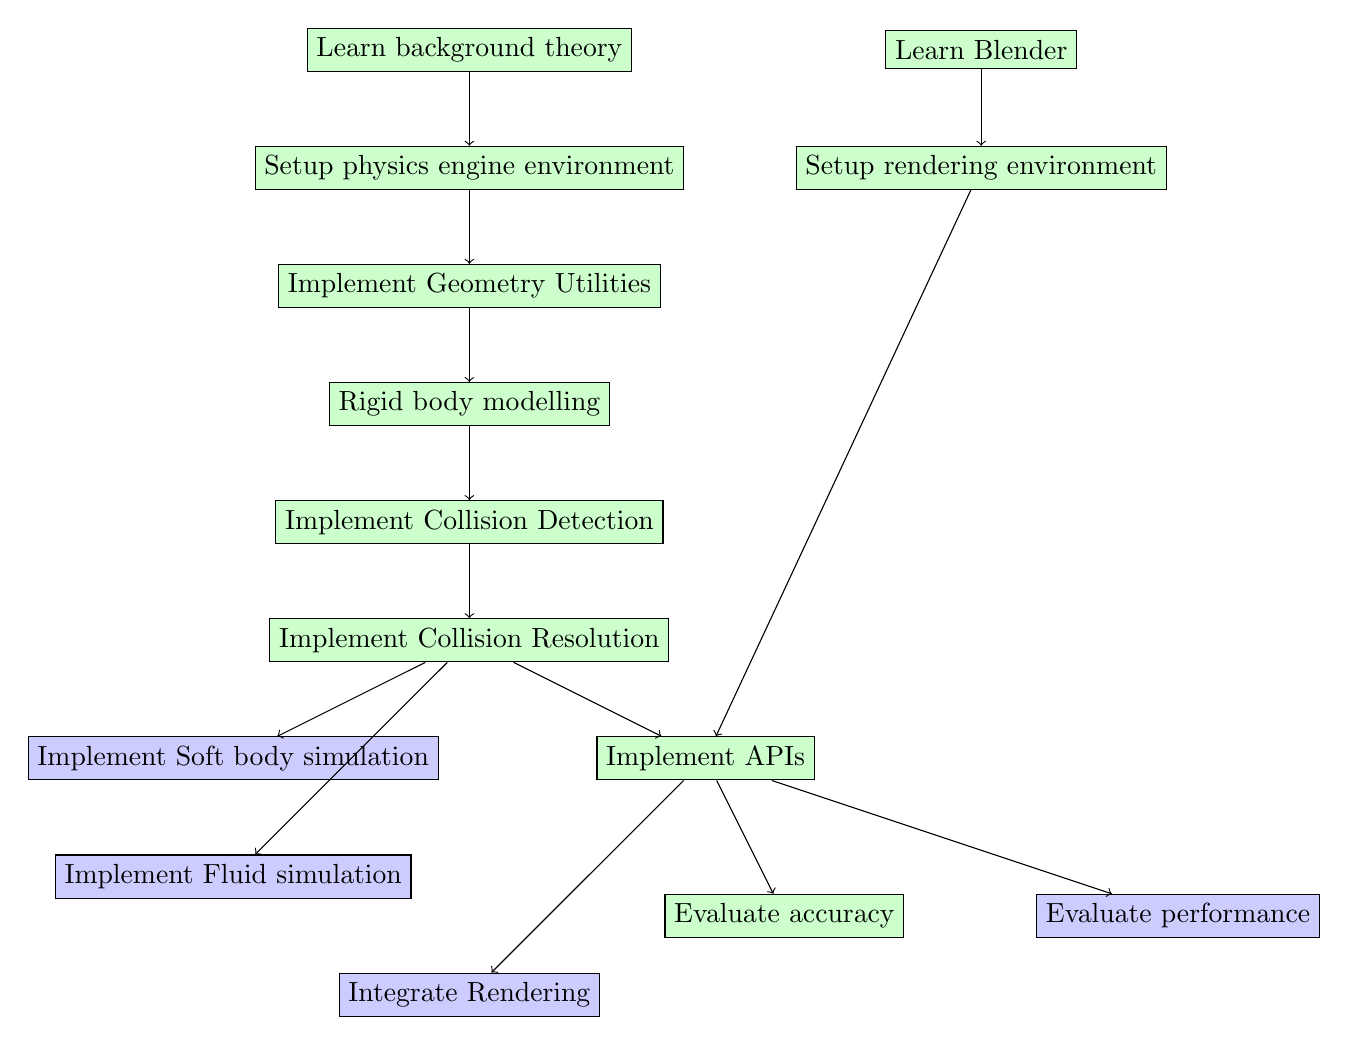
\begin{tikzpicture}
    \node [draw, fill=green!20] at (0,0) (a) {Learn background theory};
    \node [draw, fill=green!20] at (0,-1.5) (b) {Setup physics engine environment};
    \node [draw, fill=green!20] at (6.5, 0) (c) {Learn Blender};
    \node [draw, fill=green!20] at (6.5, -1.5) (d) {Setup rendering environment};
    \node [draw, fill=green!20] at (0,-3) (e) {Implement Geometry Utilities};
    \node [draw, fill=green!20] at (3, -9) (f) {Implement APIs};
    \node [draw, fill=green!20] at (0,-4.5) (g) {Rigid body modelling};
    \node [draw, fill=green!20] at (0,-6) (h) {Implement Collision Detection};
    \node [draw, fill=green!20] at (0,-7.5) (i) {Implement Collision Resolution};
    \node [draw, fill=green!20] at (4,-11) (j) {Evaluate accuracy};
    \node [draw, fill=blue!20] at (9,-11) (k) {Evaluate performance};
    \node [draw, fill=blue!20] at (-3, -9) (l) {Implement Soft body simulation};
    \node [draw, fill=blue!20] at (-3, -10.5) (m) {Implement Fluid simulation};
    \node [draw, fill=blue!20] at (0, -12) (n) {Integrate Rendering};
    \path [draw, ->] (c) -- (d);
    \path [draw, ->] (d) -- (f);
    \path [draw, ->] (f) -- (j);
    \path [draw, ->] (f) -- (k);
    \path [draw, ->] (f) -- (n);
    \path [draw, ->] (a) -- (b);
    \path [draw, ->] (b) -- (e);
    \path [draw, ->] (e) -- (g);
    \path [draw, ->] (g) -- (h);
    \path [draw, ->] (h) -- (i);
    \path [draw, ->] (i) -- (f);
    \path [draw, ->] (i) -- (l);
    \path [draw, ->] (i) -- (m);
\end{tikzpicture}
\caption{Module Dependency Analysis}
\end{figure}

\subsection{Development model}

The project mainly tackles software engineering challenges. The waterfall development model suits best for the reasons below. 

\begin{itemize}
\item The separation into different stages gives a good indication on the progress of the project throughout. 
\item The project has well defined requirements, resources and technologies, allowing the separation to be clear.
\item Balancing between the stages are very much needed, as for example spending too much time on researching is not desireable, and the implementations need to undergo testing. The division of stages reminds me to not get stuck at one step and not move on.
\item Contrast with agile development, the project focuses on building one predetermined software, so reiterations are unecessary.
\end{itemize}

During the process of the development there has been some delays in some parts, so I spent some buffer time to catch up with some difficulties, particularly in the implementation stage and dissertation writeup stage. Gantt chart \ref{ganttlbl} is also used for the planning of the project.


\begin{figure}\begin{center}\label{ganttlbl}
    \resizebox{\linewidth}{!}{%
\begin{ganttchart}{1}{30}[
    
    bar label font=\small,
    milestone label font=\small,
    group label font=\small,
    expand chart=1.2\textwidth
]
    \gantttitle{Project Progress Gantt Chart (30 Weeks)}{30} \\
    \gantttitlelist{1,...,30}{1} \\
    \ganttbar{Implementation}{1}{15} \\
    \ganttbar{Writeup}{22}{30} \\
    \ganttbar{Proposal}{1}{2} \\
    \ganttbar{Framework setup}{3}{4} \\
    \ganttbar{Implement Modelling}{5}{8} \\
    \ganttbar{Implement Collision Detection}{9}{12} \\
    \ganttbar{Implement Collision Resolution}{12}{15} \\
    \ganttbar{Evaluation}{18}{21} \\
    \ganttbar{Dissertation drafting}{22}{25} \\
    \ganttbar{Dissertation amending}{26}{30} \\
    \end{ganttchart}
    }%
\end{center}\end{figure}

\chapter{Implementation}\label{chap3}

\section{Repository Overview}

%herehereherehereherehereherehereherehereherehereherehereherehereherehereherehere
[Figure of repository structure]TBA

[Figure of modules interaction]TBA

[Figures] describes the structure of the repository. The main engine is put in the engine directory, being self-supportive on its own with encapsulated APIs for setting up experiments. The engine part is fully written in C++, and has its own structure, which will be described in section \ref{englbl}. The rendering part is isolated from the main engine because it mainly uses third-party rendering library - Blender, to render the results provided by the APIs of the physics engine. However, the rendered videos were what I heavily relied on when testing and evaluating the engine. They will be described in [section XXX]. The report directory is for storing writeup files for the project.

\section{Engine}\ref{englbl}

As a reminder, the physics engine mainly involves first modelling objects as rigid bodies, then uses a collision detection-resolution feedback loop for simulation. In the repository, these core mechanics are in the core directory. I used a geometry directory to provide utilities for computational geometry. The core directory includes 

\subsection{Geometry}

For better customizability I implemented my own geometry modules. Since the whole engine operates in 3D in every way, I could use just two classes, \code{Vector} and \code{Matrix}, in order to represent $3 \times 1$ and $3 \times 3$ tensors respectively. Some common operators are also supported for quick C++ style syntax. Some of the interfaces include

\begin{itemize}
\item \code{static Matrix star(const Vector\& v)}: the star operation that creates a matrix $A=a^*$ for any vector $a$ such that $A \cdot b = a\times b$.
\item \code{Matrix inverse()}: finding the inverse of a matrix
\item \code{Vector operator*(Vector rhs)}: multiplying matrices with vectors
\end{itemize}

\subsection{Rigid body}

The main class for individual rigid bodies is \code{RigidBody}, with each instance of it representing one unique rigid body. The states and auxilaries are also individually classed as \code{RigidBodyState} and \code{RigidBodyAuxilaries} respectively.

For each rigid body, the main fixed properties are its \code{mass} and \code{bodySpaceInertiaTensor}. I also implemented a prepared \code{CuboidRigidBody} that subclasses from \code{RigidBody}, and instead uses \code{length}, \code{width}, and \code{height} to automatically calculate the integral. The subclasses are also responsible for documenting shapes information when outputting.

In order to implement the later edge-edge or vertex-face collision detection, the collection of vertices, edges and faces are also saved and managed by the subclasses.

All the derivatives and computable auxilaries are encapsulated as methods like 

\begin{verbatim}
RigidBodyState computeDerivative(RigidBodyState state, 
RigidBodyForceAndTorque forceAndTorque)
\end{verbatim}

\subsection{Ordinary Differential Equations}

Earlier in [section TBA], the state of a rigid body, $S$, and its derivative with regards to time $t$, $\frac{d}{dt}S$, are defined with variables from states $S$ together with outside force and torque. Force and torque are assumed to be known ahead of time (they are usually a constant, for example, gravity constantly pulls everything downwards, or other user-defined constant force fields), but they also might change depending on the result of collision resolution. They can be treated as a known function of time, say $f(t)$. The derivative depends on the force and torque and the current state, so it can be treated as a known function of both of them, say $g(S, f(t))$. This helps establishing a differential equation for predicting the next states

\begin{equation}
\frac{d}{dt}S = g(S, f(t))
\end{equation}

which can now be processed as an ordinary differential equation (ODE), where the states at the current time frame $t_0$ are given, and the equation is used to find the states at the next time frame $t_0 + dt$.

I decided to use a naive approximation (known as Euler's method) by assuming the derivative remains constant across the duration of the small time frame $dt$. That is, I derived the derivative at $t_0$ as $\frac{d}{dt}S=g(S, f(t_0))$, and advance the state $S$ by simply adding $dt \cdot \frac{d}{dt}S$ to the state $S$. This in fact works very well already, considering most of my experiments expand over several seconds, so it turns out to be very difficult if not impossible for humans to notice the tiny discrepancies. It is also possible to divide to time steps even more, and with smaller steps (smaller $dt$) the accuracy will be improved even further.

There are in fact more precise simulations using an actual ODE solver. For example, there are known ODE solvers such as the Boost.ODEInt library that deploys more complicated algorithms such as fourth-order Runge-Kutta method to integrate the ODE. However, these are not considered in this project considering the original goal of the project is the ability to simulate rather than the ability to accurately approximate things. Of course, they are interesting candidates to consider as future improvement.

\subsection{Unconstrained Simulation}

Given the rigid bodies and simulation basics, the actual state advancement is as simple as going through all bodies recorded in the engine:

\begin{verbatim}
void advanceByTimeFrameUnderConstantForce(double dt) {
    for (auto body : bodies) {
        auto states = body.getStates();
        auto [time, state] = states.back();
        auto stateDerivative = body.computeDerivative(state, body.getForceAndTorque());
        states.emplace_back(std::make_pair(time + dt, state + stateDerivative * dt));
    }
}
\end{verbatim}

All the state history along with timing information is recorded and saved in a \code{std::vector} in time order. This is helpful when we need to unroll the states to a previous time frame due to collision detection.

\subsection{Collision Detection}

This stage turns out to be one of the trickier modules to implement. I implemented them directly as methods of the main \code{PhysicsEngine} class. The collision detection has several steps.

\subsubsection{Entry point} 
Collision detection methods are called immediately after advancing the previous unconstrained simulation. The problem of the previous unconstrained simulation is that it does not consider collision or interactions between rigid bodies in the engine. In fact, what we did is to advance the states no matter what happened, and check if any problems arise afterwards. The idea behind this is that collisions are rare in most scenerios, and it is common that only a couple of collisions happens throughout the experiment. Hence, we could be lazy and check for collision every $10$ steps of regular unconstrained simulation, since checking for collisions are quite resource-intensive. However there is the issue of having objects clip through each other with longer time frames of checking. In practice I called the detection after every regular unconstrained simulation since it is enough for simple experiments.

\subsubsection{Bounding boxes}
As a preprocessing step, the bounding boxes of all existing rigid bodies are generated. Bounding box is the smallest box that encapsulates the object but is also aligned with the axis, which simplifies computations. [fig] shows an example of a bounding box.

[fig]TBA

If collisions were to occur, the bounding boxes, which represent an even larger space, must collide first. So checking if two bounding boxes overlay is a good precondition for actual collisions, and does a good job of filtering out most of the non-colliding cases.

Checking if any pairs of bounding boxes overlap is much more efficient. Even a naive pairwise check between all pairs of bounding boxes are more efficient because no need to iterate over edges and faces, with a complexity of $O(n^2)$ where $n$ is the number of rigid bodies. But it can be solved more efficiently.

\begin{itemize}
\item One-dimensional case: Consider what will happen if the bounding boxes are in only one dimension. In that case, the boxes are actually simply segments. Let's say the $i$-th segment covers $l_i$ to $r_i$, and we are tasked with finding all the overlapping pairs quickly, where there are $n$ segments at the beginning, and at most $m$ pairs overlap.

[fig]TBA

This problem can be solved in $O(n \log n + m)$ time with a sweep line algorithm. First, all the endpoints ($l_i$ and $r_i$, a total of $2n$ endpoints) will be sorted from left to right. Then a sweep is performed from left to right, while keeping a list of which segments are active. When we get a left endpoint $l_i$, the segment is marked as active, and it will be paired with all other active segments. When we get a right endpoint $r_i$, the corresponding segment is removed from the active list. The list needs to support quick insertions and deletions, so a doubly linked list for example would suffice. The initial sorting costs $O(n\log n)$, the sweep costs $O(n)$, going through the pairs costs $O(m)$, adding to a cost of $O(n\log n + m)$, and is the most efficient algorithm for solving this problem.

After solving this initial problem at the first time frame, the subsequent problems for later time frames can be slightly improved based on the assumption that they do not greatly deviate from the original problem. The bottleneck in the algorithm is the sorting of the endpoints. We could use the idea of insertion sort here - for each endpoint, check if it is to the right of the previous endpoint, and if not swap its position with the previous endpoint. Now the complexity becomes $O(n + s)$ where $s$ is the number of swaps. Although in the worst case scenerio $s$ could be as high as $O(n^2)$, we could expect $s$ to be low on average. After re-sorting all the endpoints, the sweep step could continue as before, yielding $O(n + m + s)$ in total.

But we could even do better, by not performing the sweep step at all! Let's assume the whole list of overlapping segments is recorded. Consider when a pair of segments, $i$ and $j$, change from overlapping to not overlapping. Then, the relative order of the four endpoints $l_i$, $r_i$, $l_j$, $r_j$ must have changed. So when doing the pesudo insertion sort, two of those four values must have swapping places with another when adjacent. Same goes when $i$ and $j$ change from not overlapping to overlapping. Therefore, whenever we perform a swap, we should re-check the overlapping status of the pair of underlying segments have changed. Now we successfully eleminated the need for sweeping phase, yielding a total complexity of $O(n + s)$.

\item Three-dimensional case: Now going back to our 3D bounding boxes. There are efficient algorithm with advanced data structures that solve the one-time problem in $O(n\log n + m)$ as well. A general result is for $d$ dimensions the overlapping pairs can be found in $O(n \log ^ {\max(1, d - 2)} n + m)$.

For subsequent steps, a similar optimization could be used. This time, the boxes have three sets of segments: $xl_i, xr_i, yl_i, yr_i, zl_i, zr_i$. Thankfully checking whether two bounding boxes overlap is still $O(1)$. So similarly, consider when a pair of boxes, $i$ and $j$, change from overlapping to not overlapping or vice versa. The relative order of four endpoints on at least one axis must have changed. Therefore, if we simply maintain three sorted lists of each dimension, and perform a pesudo insertion sort for each of them with re-checking if pairs of bounding boxes still overlap, the whole list of overlapping bounding boxes is still maintained at a manageable $O(n + s)$ complexity.
\end{itemize}

\subsubsection{Collision}

Collisions are only further checked on overlapping bounding boxes. Each collision is recorded as a class:

\begin{verbatim}
class Collision {
    RigidBody *a, *b;
    Vector normal;
};
class FaceVertexCollision : public Collision {
    Face face;
    Vector vertex;
};
class EdgeEdgeCollision : public Collision {
    Edge ea, eb;
};
\end{verbatim}

The two types of collisions are both accounted for. Degenerated cases like vertex-vertex collision will be described with the more general collision case. For face-vertex collison, I force \code{RigidBody *a} to be the body with the face and \code{RigidBody *b} to be the body with the vertex. The \code{Vector normal} describes the normal vector of the separating plane at the point of collision, which is either the face for face-vertex collision or the cross product of the two edges in the edge-edge collision case. All the coordinates here should use the world space coordinates. The process of collision checking is as simple as going through all possible pairs of faces-vertices and edges-edges, and checking if they have penetrated. 

The test for penetration is done by simply testing the relative velocity defined previously, $v_{AB}$, against some constant threshold.

There are also optimization possibilties here. For example, it is possible to cache the history of collisions between a specific pair of rigid bodies. Therefore, when checking for a new collision, we could first check if previous collision setups work, say if the same pairs of edges could separate them apart. If the check fails, we can first try to replace them with adjacent faces or edges, hoping that it only barely rotated. Currently these ideas are left as possible future improvements.

\subsubsection{Finding the time of collision}

Binary search could be used to find the exact time the collision takes place, assuming one already happens. If there are multiple pairs of collisions with the time frame $t_0$ to $t_0 + dt$, we are interested in finding the one that occurs first.

The idea of the binary search is to first fix the possible range, in this case the range $t_0$ to $t_0 + dt$. Previously we have discussed how to efficiently check if a collision happened at any time frame $t$. Therefore, the midpoint of the range can be queried to narrow down the possible range, up until a desired precision:

\begin{verbatim}
left = t0;
right = t0 + dt;
eps = 1e-5;
while (right - left > eps) {
    middle = (left + right) / 2.0;
    engine.advanceByTimeFrameUnderConstantForce(middle - left);
    if (engine.checkCollision())
        right = middle;
    else
        left = middle;
    engine.rollBack();
}
\end{verbatim}

This gives a complexity of $O((n + s) \cdot \log \frac{dt}{eps})$.

\subsection{Collision Resolution}

Most of the computations are already given in the previous section [section TBA]. Here, we just plug in the computations for the relevant quantities. In the code, it can be encapsulated as a simple method \code{resolveCollision(Collision *c, double coefficientOfResititution)}, where the collision is resolved by supplying the collision and the coefficient of resititution. 
In the actual implementation I chose a default value for the coefficient as $\epsilon = 0.5$. 

Now, after correcting the states of all rigid bodies, the states will be saved as a special time frame, and the simulation will resume in a physically correct manner.

\section{Render}

Strictly speaking the rendering step is out of the scope of the actual project here, because the users could just invoke the APIs of the core engine and get whatever data they would like to collect. However, it has ultimately become an important step of the project with the need to perform experiments and visualize simple simulations. This is also where a lot of trouble shows up for my project which ultimately stems from my poor knowledge of rendering libraries prior to this project.

\subsection{Motivation}

I chose Blender because it is known as a very popular 3D rendering program. It turns out that it is popular for being friendly to people with little programming knowledge, with a good UI, but not particularly great for dumping external data in for it to render whatever I want. It seems that the only relevant functionality for this purpose is to use the Blender python scripting API, which, while has some documentations and some powers, aren't as well-studies as other functionalities of Blender, since it is still under active development and refinement. In fact, the documentation just updated to 4.1 [TBA ref] within the duration of the project from 4.0.

\subsection{Native python scripting}

Blender scripting works with a custom module provided by Blender as the rendering module. However, it does not work like other common, distributed modules like matplotlib - the module is provided in a native python version inside Blender, hidden in the source directory.

In order to use it, most of the rendering related scripts have to be built on top of this native environment, which cannot be easily manipulated as common python distributions. For example, installing new libraries like scipy need to be done directly with the pip installer on the native python environment.

I ended up using a setup script to deal with all the nuances by directly specifying the \code{\%BLENDERPATH\%}, include the python in the \code{\%PATH\%} together with libraries installations, and then return to the current directory for running the script.

\subsection{Rendering process}

It took me some time to learn how to setup the rendering stage. First, the camera needs to be setup with an appropriate bounding box. Then, remove all existing objects in the stage, because for some reason some of the objects could persist to the next run. With each rigid body, create a separate mesh for them, add animation data for them, and interpolate the animation with the key data at each time frame from our simulation data. Finally, setup the rendering options and render the animation to a video.

There are also many details regarding each animation data. For example, the rotation used by Blender is the quanternion one. Quanternion functions as an alternative to the matrix form of rotation. Luckily \code{scipy.spatial.transform} provided translations between matrix form and quanternion form.

\subsection{Pipeline}

Finally, I created a way to pipe the data the engine outputs to be directly used by the blender python script. I used C++ code to setup the experiment, build it with cmake and makefile, which should automatically dump the data into the rendering directory. Then I head into the rendering directory and use my setup script to render the result as a video. It turns out the rendering could take a very long time, for reference a 10 second video ends up renderng for 10 minutes. To adapt to this I tried to work with small and simple experiment setups to perform some quick testings.



\chapter{Evaluation}\label{chap4}


Evaluation of physics engines in general can be quite challenging, 
especially for quantitative analysis.
Little work has been done in this area as of now, 
likely due to the complexity, systematic bias, and the lack of needs.

The evaluation of this project is split into three parts: Benchmark selection, Quantitative evaluations, and Success criteria.

\section{Benchmark selection}

Quantitative evaluations will be largely comparison-based. 
I will be choosing two open-source physics engines that support similar features to compare against.
The following engines have been found as possible candidates:

\begin{table}[h]
  \centering
  \makebox[\linewidth]{
  \begin{tabular}
  {|c|c|}
  \hline 
  Physics engine                                & Website                                                         \\
  \hline 
  Advanced Simulation Library                   & asl.org.il                                           \\
  Bullet                                        & pybullet.org                                           \\
  Newton Game Dynamics                          & newtondynamics.com/forum/newton.php                      \\
  Open Dynamics Engine                          & www.ode.org                                            \\
  PAL              & www.adrianboeing.com/pal                                \\
  PhysX                                         & www.nvidia.com/en-gb/geforce/technologies/physx        \\
  Project Chrono~                               & projectchrono.org                                      \\
  Siconos                                       & nonsmooth.gricad-pages.univ-grenoble-alpes.fr/siconos  \\
  SOFA & www.sofa-framework.org                                 \\
  Tokamak physics engine                        & github.com/isegal/TokamakPhysics                        \\
  \hline
  \end{tabular}
  }
\end{table}

They have then been further narrowed down in consideration of supportability, documentation and popularity. I end up choosing the following physics engines as benchmarks:

\begin{table}[h]
  \centering
  \makebox[\linewidth]{
  \begin{tabular}
  {|c|c|}
  \hline 
  Physics engine                                & Reason???TBA, +screenshots, +brief description on setups                                                         \\
  \hline 
  PhysX                                         & www.nvidia.com/en-gb/geforce/technologies/physx        \\
  SOFA & www.sofa-framework.org                                 \\
  \hline
  \end{tabular}
  }
\end{table}


\section{Quantitative evaluations}

The functionalities of selected physics engines along with mine will be evaluated through a series of small runtime tests.
The tests partially drew inspiration from other existing researches on physics engines\cite{seugling2006evaluation}.

\subsection{Bounce test}

\subsubsection{Setup}

To test whether the engines could handle object collisions, I measure if the momentum and energy are preserved.

Two identical cubes will be placed in a world with no gravity. 

Cube A, the one on the left, is located at $(0, 0, 0)$, and is moving along the \code{+x} direction with a velocity of $\SI{1}{\m\per\s}$.

Cube B, the one on the right, is located at $(\SI{5}{\m}, 0, 0)$, and is moving along the \code{-x} direction with a velocity of $\SI{1}{\m\per\s}$.

Both cubes are 1x1x1 and have a mass of $\SI{1}{\kg}$. The coefficient restitution $\epsilon$ is a variable that ranges between $0$ and $1$.

\begin{center}
  \makebox[\textwidth]{\includegraphics[width=\textwidth]{figs/img1.png}}
\end{center}

Theoretically, the sum of momentum vectors should stay at $(0, 0, 0)$, and the total energy at $\SI{1}{\J}$.
The actual sum of momentum and total energy, as simulated by the engine, will be plotted against time.
The less these values vary, the more accurate the simulation is.

\subsubsection{Result}

All perfectly correct, for all engines. [fig]TBA

As seen in [fig], both the sum of momentum and the total energy stay true to the theoretical results with no noticeable inaccuracies. This is a very basic bouncing task, so as expected all physics engines could reliably accurately simulate it.

\subsection{Support test}

\subsubsection{Setup}

A box will be placed on a fixed inclined plane. The coefficient restitution $\epsilon$ is set to be $0$ - this means a perfectly inelastic collision happens between the box and the plane, so the plane should be able to support the ball. Test if the ball could slide down the plane in an accurate manner. In order to simulate the plane being "fixed" while still being a cuboid rigid body, its mass will be set to infinite, and will be carefully placed with some initial rotation.

The plane passes through the origin $(0, 0, 0)$ and is sufficiently long to hold the cube. The experiment is mostly within the $x-z$ plane. The cube is 1x1x1, and its center of mass is placed at $(-20\cos \theta + \frac{1}{2}\sin \theta, 0, 20\sin\theta+\frac{1}{2}\cos \theta)$. This means its middle contact point with the plane is always $d=20$m from the origin. Constant gravity $G = \SI{10}{\N}$ will be applied to the cube. At any none $0$ degree angle $(\theta > 0)$, the cube should slide down the plane. The time it takes for the $x$ coordinate of its centre to reach $\frac{1}{2}\sin \theta$ will be measured and checked with the theoretical result. Then the experiment will be repeated for different angles $\theta$ within the range $(0, \frac{\pi}{2})$.

In order to obtain a theoretically perfect result, consider a cube moving frictionless slope. Its acceleration along the slope should be $a=\frac{G}{m}\sin \theta$. If the time it takes when accelerating from a static position is $t$, the distance travelled should be $\frac{1}{2}at^2$. So the theoretical time it takes to reach the origin should be $t_0=\sqrt{\frac{2d}{a}}=\sqrt{\frac{2dm}{G\sin \theta}}=\frac{2}{\sqrt{\sin\theta}}$.

\begin{center}
  \makebox[\textwidth]{\includegraphics[width=0.5\textwidth]{figs/img2.png}}
\end{center}

\subsubsection{Result}

TBA
5, 7.2, 7.433
10, 5.04, 5.167
20, 3.5, 3.633
30, 2.88, 2.900
40, 2.54, 2.567
50, 2.32, 2.333
60, 2.18, 2.233
70, 2.08, 2.133
80, 2.04, 2.100
85, 2.02, 2.067

As seen in [fig], in general the time it takes for the cube to slide down matches with the theoretical result, but in general all the engines give a slightly higher result. This is likely due to accumulated inaccuracies of repeated collisions along the slope. From the view of a physics engine, the cube repeated collides with the slope, and the result is its downwards momentum transfers into sliding momentum. The transfers needed to be calculated every time, so it could be slightly delayed compared to the theoretical analysis.

\subsection{Pendulum test}

\subsubsection{Setup}

Have a pendulum setup like in the following figure.

A small object is attached to a fixed point using a "thread" with a length of $L=\SI{10}{\m}$. To simulate such a "thread" in my physics engine, the object is simply "pulled" back up after unconstrained simulation at each time step.

The initial angle between the bar that connects the sphere and an imaginary vertical line through the fixed point is $\theta$.

\begin{center}
  \makebox[\textwidth]{\includegraphics[width=0.3\textwidth]{figs/img3.png}}
\end{center}

$\theta$ is gradually increased from $5 \degree$ to $85 \degree$.
For each $\theta$, 
the period of the pendulum is measured by recording the time it takes for the sphere to reach its lowest point $5$ times.

Theoretically, the period of a pendulum is

\begin{equation}
T = 2  \pi \cdot \sqrt{\frac{L}{g}}
\end{equation}

The periods as simulated by the engines will be plotted against the angle $\theta$.

\subsubsection{Result}

TBA
5, 18.24 (/ 2.5)
10, 18.30
20, 18.26
30, 18.26
40, 18.30
50, 18.36
60, 18.46
70, 18.58
80, 18.80
85, 18.93

As seen in [fig], this is an experiment where all the physics engine deviate quite a bit from the theoretical results. Engines generally take a longer time to swing the pendulum as the degree increase, possibly due to the accumulation of correction errors from the thread constraining the object, which should have resulted in an arc, but got simulated as small segments.

\section{Success criteria}

Success criteria from the project proposal:

\begin{itemize}

\item Implement all basic modules: Object modelling, Collision detection, Bounce, Friction, Stability.

\item Evaluate the engine by comparing it with popular existing engines with simple experiments.

\item Demonstrate that the engine works with screenshots of simple examples.
\end{itemize}

For extensions (ordered by priority):

\begin{itemize}
\item Implement fluid dynamics.

\item Implement different versions of the engine for whether GPU is used, and for other interesting parameters like the number of cores used. 
Then evaluate the performance.

\item Implement real-time rendering, which should allow the project to meet all previous criteria without third-party rendering libraries. 

\item Implement soft-body dynamics.

Referring back to the success criteria, I consider all core criteria to be completed and successful. Extensions were attempted but not as successful. All basic modules related to rigid body simulation are implemented and evaluated with simple experiments. The followings are some example screenshots of the resulting rendered video.

\begin{center}
  \makebox[\textwidth]{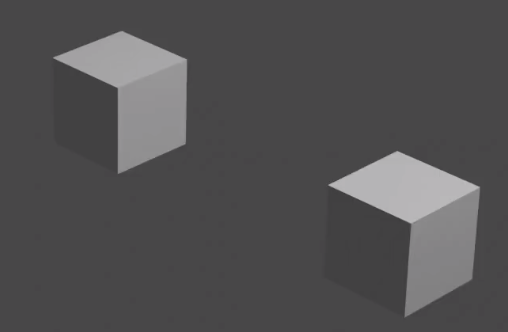
\includegraphics[width=\textwidth]{figs/sc1.png}}
\end{center}

[fig]

The results of the evaluations also show a high correlation with real-life physics results. Therefore, my physics engine is indeed capable of simulating simple rigid body interactions.

\subsection{Limitations}

As seen from some of the experiments TBA[ref], the inaccuracies of simulating certain interactions are slightly greater than popular existing physics engine. Furthermore, external functionalities, configurable options, API documentations and bug considerations are definitely not as complete as other popular physics engines. Most modern physics engines provide several alternate simulation methods, for example for solving differential equations mentioned in TBA[ref]. Some extensions like liquid simulation are also not in a working state in my engine but is supported by many other engines. On the other hand, they possess dedicated maintenance by large groups of developers, so it is not reasonable to aim at surpassing their massive project in every possible way.

\end{itemize}

\chapter{Conclusion}\label{chap5}

\section{Achievements}

The built physics engine has successfully achieved all of the success criteria. Firstly, a simple physics engine was developed to accurately simulate rigid body dynamics, incorporating efficient collision handling mechanisms. Subsequently, by leveraging the capabilities of the rendering software Blender, various functionalities of its APIs were tested by conducting small experiments within the context of rigid body simulation. These experiments yielded demonstrable instances of successful simulations, as a way of showcasing the working state of the implemented physics engine. A comparative analysis with several publicly available physics engines were done based on these experiments, where the accuracy of the evaluation was measured and compared. The results showed that my physics engine consistently simulated similar results to these counterparts, therefore confirming its ability in the field of rigid body dynamics.

\section{Lessons learnt}

A very core part of this project throughout was software engineering. Having little experience with building upon actual hefty software projects, I found a lot of the challenges in this area. Some particular challenges I would like to highlight are:
\begin{itemize}
\item Using an automated build system with CMake and Makefile.
\item Organizing a project repository.
\item Using OOP concepts with C++ development.
\item Devising computational geometry formulation.
\item Algorithm designs for simulation.
\item Deploying third-party software (Blender) in the project.
\item Incorporating two different languages.
\end{itemize}

Outside of software development and the zeros and ones, my project management skill is also significantly tested with a medium length project. It turns out to be very difficult to balance project with regular life, and all the time constraints and meetings with supervisors also add quite a bit on the challenge. I end up running a bit low on time for the extensions and the dissertation writing, which is definitely a foreseeable mistake from the current view point. At the same time, I honed my academic report writeup ability with a project I knew the most about.

For lessons more specific about my project, I find numerical debugging takes a ton of efforts, and it is very important to clear up the mind and get the initial calculation correct. The problem especially exacerbated with a somewhat shaky debugging method, and the time to take a test run and find the issues went higher than expected without very careful unit testings. I would consider laying down more unit testing code before ending up with an interconnected calculation mess for future projects like this.

\section{Future work}

I have many ideas for potential future work directions. They were not realistic due to the time constraints of the project submission, and some were mentioned before [TBA].

\begin{itemize}
\item Wider project aim: The built physics engine is primarily a personal project too simple for actual industry use without more optimizations and support. If time allows, the project could be more ambitious and aims at more recent ideas, for example making the whole physics engine differentiable to allow maching learning tunings mentioned in recent papers\cite{degrave2019differentiable}. 
\item Better project structure: I used a render outside of the proposed physics engine for most of the debugging and visualization. The rendering software is better to be in-house than external, and debugging should have been separated from visualization. Ideally, there should be dedicated testing code for unit testing the functionalities separately, which would further reduce the number of bugs and issues in the project.
\item Collision Checking Optimization: There are several subtle optimizations for collision detection. Scanning through potential pairs of rigid body is already a very interesting topic, and meanwhile my project explored an $O(n + s)$ per check idea, there could be other efficient algorithms to consider. Another possibilty I mentioned but didn't bother to implement is caching the pair of components that cause the collision from a previous timestamp, and using it to quickly check if the collisions just move to an adjacent compoent. This means storing vertices, edges, and faces in an ordered manner, and the closer two things are the more likely it is that in the case of collision they could both be separating plane candidates.
\item Differential Equation: I used a simple Euler's method to advance the timestamp after deriving the derivatives. However, this is a very research-heavy topic, and various new methods have been put forward for accurately solving the differential equation for different contexts. Some recent work about this put forward the possibilities of data reinforcement\cite{koch2021data} as a possibilty.
\item More extensive modules: I mostly focused on rigid body simulation for this project and had little time to proceed on other possible modules to add to my physics engine. There are many other considerations, and despite many of them being very difficult and being currently open to research, I would still be interested to see how incorporating them on top of my rigid body simulation system would go. Some potential ideas to consider are \cite{vinuesa2022enhancing}, \cite{obiols2020cfdnet}, \cite{li2022contact}, some of which proposing the incorporation of several machine learning methods.
\item Open software packaging: Finally, as a way of contributing to actual public, it would be preferrable to have the project deliverable through open software means like GitHub. It would allow much more engagement for future support that directly focuses on target users, and thus set a more meaningful goal in the open source community.
\end{itemize}

%%%%%%%%%%%%%%%%%%%%%%%%%%%%%%%%%%%%%%%%%%%%%%%%%%%%%%%%%%%%%%%%%%%%%
% the bibliography
\addcontentsline{toc}{chapter}{Bibliography}
\bibliography{refs}
%%%%%%%%%%%%%%%%%%%%%%%%%%%%%%%%%%%%%%%%%%%%%%%%%%%%%%%%%%%%%%%%%%%%%
% the appendices
\appendix

\chapter{Project Proposal}
\label{proposallbl}
\documentclass[12pt]{article}
\usepackage{graphicx, indentfirst, tikz, gensymb, url} % Required for inserting images
\usepackage[load-configurations = abbreviations]{siunitx}
\def\checkmark{\tikz\fill[scale=0.4](0,.35) -- (.25,0) -- (1,.7) -- (.25,.15) -- cycle;} 

\title{Building a Physics Engine From Scratch}
\author{js2657}
\date{Oct 2023}

\begin{document}


Proposal Draft V2

Building a Physics Engine From Scratch

Supervisor: Joe G March

UTO: Rafal Mantiuk

TODO:

0: Typeset \checkmark

1: Add references \checkmark

2: Grammar check \checkmark

3: Expand on extensions \checkmark

4: Add Evaluation section \checkmark

5: Add tables and images \checkmark

Issues:

0: One main issue is, how should I deal with success criteria?
On the one hand, I agree with Richard's feedback that saying something too explicit is dangerous, 
and sometimes discouraging due to being unrealistic to compare such a project with real-life huge projects.
On the other hand, many people seem to have expected some definitive success criteria to be stated.
This is showed through the checker feedback, as well as many past project proposals where there are many examples of 
"I will achieve significantly better results than X"

1: Is the current evaluation perhaps a bit too specific?

Checker feedback:

you need to put the actual references, as they would help us understand the context of your project.
\checkmark

As stated in phase I, you need to identify a UTO/supervisor who would help you shape the proposal
\checkmark

Give that there are a lot of open source physics engines, I am not convinced that developing your own will address their shortcoming that the computations are done under the hood. Need to have a different motivation
\checkmark

It is good that you will be comparing against existing engines. What will you be looking for in this comparison? What will be the success criteria for your project? You need to define these ASAP.
[Refer to issue 0]

Also pick one or two extensions and expand on them to ensure that we have a good plan for the project.\checkmark

DoS feedback:

My main feedback on this is that you need to have some evaluation in your core. 
You should decide what that is and specify it explicitly.
A bit more specifically I mean.
So would give some examples of how you intend to quantitatively compare your engine to others.
\checkmark

As a point of style I'd use 'heuristics' instead of 'hacky methods' 
\checkmark

And I would recommend explicitly stating that you're going to model velocity and angular velocity of rigid bodies in your core. 
(I know you say it in the description; but would include it again for good measure)
\checkmark

I think the references are missing too
\checkmark

Also fix the latex section numbers to avoid the '0.n' thing 
\checkmark


\section{Introduction}

Physics Engine, a term frequently used in video game industry and science research, 
is a tool that simulates physical phenomena using a computer.
The first computer, ENIAC, at one point used a physics engine to help design military weapons\cite{rojas2002first}.
At the core of physics engine, semi-realistic results are obtained through a combination of 
computation-efficient numerical approximations, 
careful modelling of the objects, 
and sometimes clever hacks that enable the engine to just make the cut.

There are some common terminologies in physics engines.
\begin{itemize}
\item \textbf{Rigid body} is an individual object that will be simulated in the engine.
A rigid body is an object that does not distort or bend, as opposed to soft body or fluid, 
which gives rigid bodies the benefit of simplicity.
A typical physics engine needs to keep track of its mass, position, orientation, linear velocity, angular velocity and impulse.
\item \textbf{Collider} is a part of a rigid body.
Complex rigid bodies tend to get separated into simple, convex colliders like spheres and boxes in the pipeline.
\item \textbf{Collision detection} and \textbf{Collision resolution} are components of the engine which handle the interaction between colliders.
Commonly physics engine continuously advances the time by a small fraction of a second, moving the objects according to their speed.
After each position update, Collision detection will kick in and detect if a pair of colliders will intersect.
If so, Collision resolution will decide whether and how they will get bounced and separated apart, 
updating their velocities accordingly.
\end{itemize}

Many open-source physics engines are available online, including PhysX\cite{physx}, 
Box2D\cite{box2d} and Bullet\cite{bullet}.
However, the most common way a physics engine is presented is as a big, mysterious library 
where all the computation is done under dozens of dependencies and documentation.
As a result, adding a simple feature could take a lot of effort of plowing through documentation and files.
I want to build my own physics engine, 
which gives me the flexibility to add whatever I want because I would know exactly how it works.

\section{Description}

My project aims to build a 3D real-time physics engine from scratch that implements basic modules, 
without making use of any currently available physics engine.
My focus will be to realise the visual effects rather than being extremely accurate or efficient,
considering the limited time, my available hardware resources, and the ease of experiments and showcases.
This is also why I chose to build a real-time physics engine over a high-precision one.
In addition, this project will also provide a basic framework that is easy to extend upon in the future, if necessary.
Overall, this project will be a great opportunity for me to learn more about physics and programming.

Here is a list of the basic core modules I plan to implement:
\begin{itemize}
\item Object modelling: Create data structures for recording attributes of rigid bodies and design interfaces for applying forces and adding colliders.
Typical physical attributes of rigid bodies include mass, position, orientation, linear velocity, angular velocity, and impulse.
\item Collision detection: Adopt many algorithms to decide if collisions happen.
\item Bounce: Part of Collision resolution where some maths are used to find the approximated results of a bounce.
\item Friction: Part of Collision resolution where vast assumptions are used to simulate real-life friction.
\item Stability: Part of Collision resolution where some heuristics are used to prevent certain visual artefacts.
For example, if two objects are stacked together, the upper one should not be bouncing up and down constantly.
\end{itemize}

The project could then be evaluated by comparisons using simple experiments against existing popular physics engines.
More on this in the Evaluation section.

Extension modules I plan to look at include:
\begin{itemize}
\item Fluid simulation:

Fluid simulation involves approximations to fluid equations, 
and can have different levels of complexity depending on the topic.
For example, 
the simulation of buoyant force of hard objects submerged in water will be simpler than 
the simulation of the flow of the fluid.
I will try my best to cover as much in fluid simulation as I can.

\item Real-time rendering:

For the sake of showcasing, I might be using existing rendering libraries like Blender\cite{blender}, 
but it is certainly better to not rely on them.

\item Performance evaluation

I will give different implementations for CPU and GPU, 
which will then allow me to draw comparisons about their contributions to performance.

\item Soft-body simulation

Unlike rigid bodies, the shape of objects can change to a certain degree.
Therefore, it is much harder to model them and deal with collisions.
I will need to do research and choose what to implement. 

\end{itemize}

\section{Evaluation}

Evaluation of physics engines can be quite challenging, 
especially when quantitative analysis is preferred.
Little work has been done in this area as of now, 
likely due to the complexity, systematic bias, and the lack of needs.

The evaluation of this project is split into three parts: Benchmark selection, Core functionality, and Performance evaluation.

\subsection{Benchmark selection}

Since the functionality evaluations will be largely comparison-based,
I will be choosing at least three open-source physics engines that support similar features to compare against.
The following engines have been found as possible candidates:

\begin{table}[h]
    \centering
    \makebox[\linewidth]{
    \begin{tabular}
    {|c|c|}
    \hline 
    Physics engine                                & Website                                                         \\
    \hline 
    Advanced Simulation Library                   & asl.org.il                                           \\
    Bullet                                        & pybullet.org                                           \\
    Newton Game Dynamics                          & newtondynamics.com/forum/newton.php                      \\
    Open Dynamics Engine                          & www.ode.org                                            \\
    PAL              & www.adrianboeing.com/pal                                \\
    PhysX                                         & www.nvidia.com/en-gb/geforce/technologies/physx        \\
    Project Chrono~                               & projectchrono.org                                      \\
    Siconos                                       & nonsmooth.gricad-pages.univ-grenoble-alpes.fr/siconos  \\
    SOFA & www.sofa-framework.org                                 \\
    Tokamak physics engine                        & github.com/isegal/TokamakPhysics                        \\
    \hline
    \end{tabular}
    }
\end{table}

I plan to further narrow them down by testing if they work in my environment, 
if they have sufficient documentation, 
and if they support the features I am going to compare on.

\subsection{Core functionality}

The functionality will be evaluated through a series of small runtime tests.
The tests are similar to the ones that already existed\cite{seugling2006evaluation}.
Please note that they are preliminary and might be adjusted for clearer visuals.

\subsubsection{Bounce test}

To test whether the engines could handle object collisions, I measure if the momentum and energy are preserved.

Two identical spheres will be placed in a world with no gravity. 
Sphere A, the one on the left, is located at $(0, 0, 0)$, and is moving along the $+$x direction with a velocity of $\SI{1}{\m\per\s}$.
Sphere B, the one on the right, is located at $(\SI{10}{\m}, 0, 0)$, and is moving along the $-$x direction with a velocity of $\SI{1}{\m\per\s}$.
Both spheres have a radius of 1m and a mass of $\SI{1}{\kg}$. The restitution will vary between $0$ and $1$.

\begin{center}
    \makebox[\textwidth]{\includegraphics[width=\textwidth]{img1.png}}
  \end{center}

Theoretically, the sum of momentum vectors should stay at $(0, 0, 0)$, and the total energy at $\SI{1}{\J}$.
The actual sum of momentum and total energy, as simulated by the engine, will be plotted against time.
The less these values vary, the more accurate the simulation is.

\subsubsection{Friction test}

Coulomb's Law describes the friction force with the coefficient of friction, $\mu$, which is a constant property of the surface.
If the friction force is $F_f$, the normal force exerted by the surface is $F_n$, then it holds that

\begin{equation}
F_f \leq \mu \times F_n
\end{equation}

Therefore,

\begin{equation}
\frac{F_f}{F_n} \leq \mu
\end{equation}

A box will be placed on a static inclined plane, whose coefficient $\mu = 0.5$.
The angle the surface is tilted by, theta, will gradually increase from 0 to $\frac{\pi}{2}$
A cube of $\SI{1}{\m} \times \SI{1}{\m} \times \SI{1}{\m}$ will be placed on that plane.
A force of gravity $G = \SI{10}{\N}$ will be applied to the cube.

\begin{center}
    \makebox[\textwidth]{\includegraphics[width=0.5\textwidth]{img2.png}}
  \end{center}

For each angle $\theta$, forces $F_f$ and $F_n$ will be computed as follows.

The normal force is equal to the proportion of gravity perpendicular to the surface:

\begin{equation}
F_n = G \times \cos \theta
\end{equation}

The friction force is calculated using Newton's First Law:

\begin{equation}
F_f = m \times a - G \times \sin \theta
\end{equation}

Now, $\frac{F_f}{F_n}$ will be plotted against the angle theta. According to Coulomb's Law, it should always stay below $\mu = 0.5$

\subsubsection{Pendulum test}

Have a pendulum setup like in the following figure.
A sphere of radius 1m is attached to a fixed point using a bar of radius $\SI{0.001}{\m}$ and length of $\SI{10}{\m}$.
The initial angle between the bar that connects the sphere and an imaginary vertical line through the fixed point is $\theta$.

\begin{center}
    \makebox[\textwidth]{\includegraphics[width=0.3\textwidth]{img3.png}}
  \end{center}

Theta is gradually increased from $5\degree$ to $85\degree$.
For each theta, 
the period of the pendulum is measured by recording the time it takes for the sphere to reach its lowest point $100$ times.

Theoretically, the period of a pendulum is

\begin{equation}
T = 2  \pi \cdot \sqrt{\frac{1}{g}}
\end{equation}

The periods as simulated by the engines will be plotted against the angle theta.

\subsection{Performance evaluation}

This part is considered as an extension. The performance will similarly be measured with a test.

There will be comparisons between my engine and other benchmark engines, as well as between different implementations of my engine.

\subsubsection{Falling test}

a total number of $n$ cubes, all of size $\SI{1}{\m} \times \SI{1}{\m} \times \SI{1}{\m}$, 
are placed at $(0, 0, \SI{2}{\m}), (0, 0, \SI{4}{\m}), \ldots, (0, 0, (n \times 2)\SI{}{\m})$ above a plane of $z = 0$, 
as shown below.
The masses of each cube is chosen uniformly between $\SI{1}{\kg}$ to $\SI{10}{\kg}$, in order to add complexity.

\begin{center}
  \makebox[\textwidth]{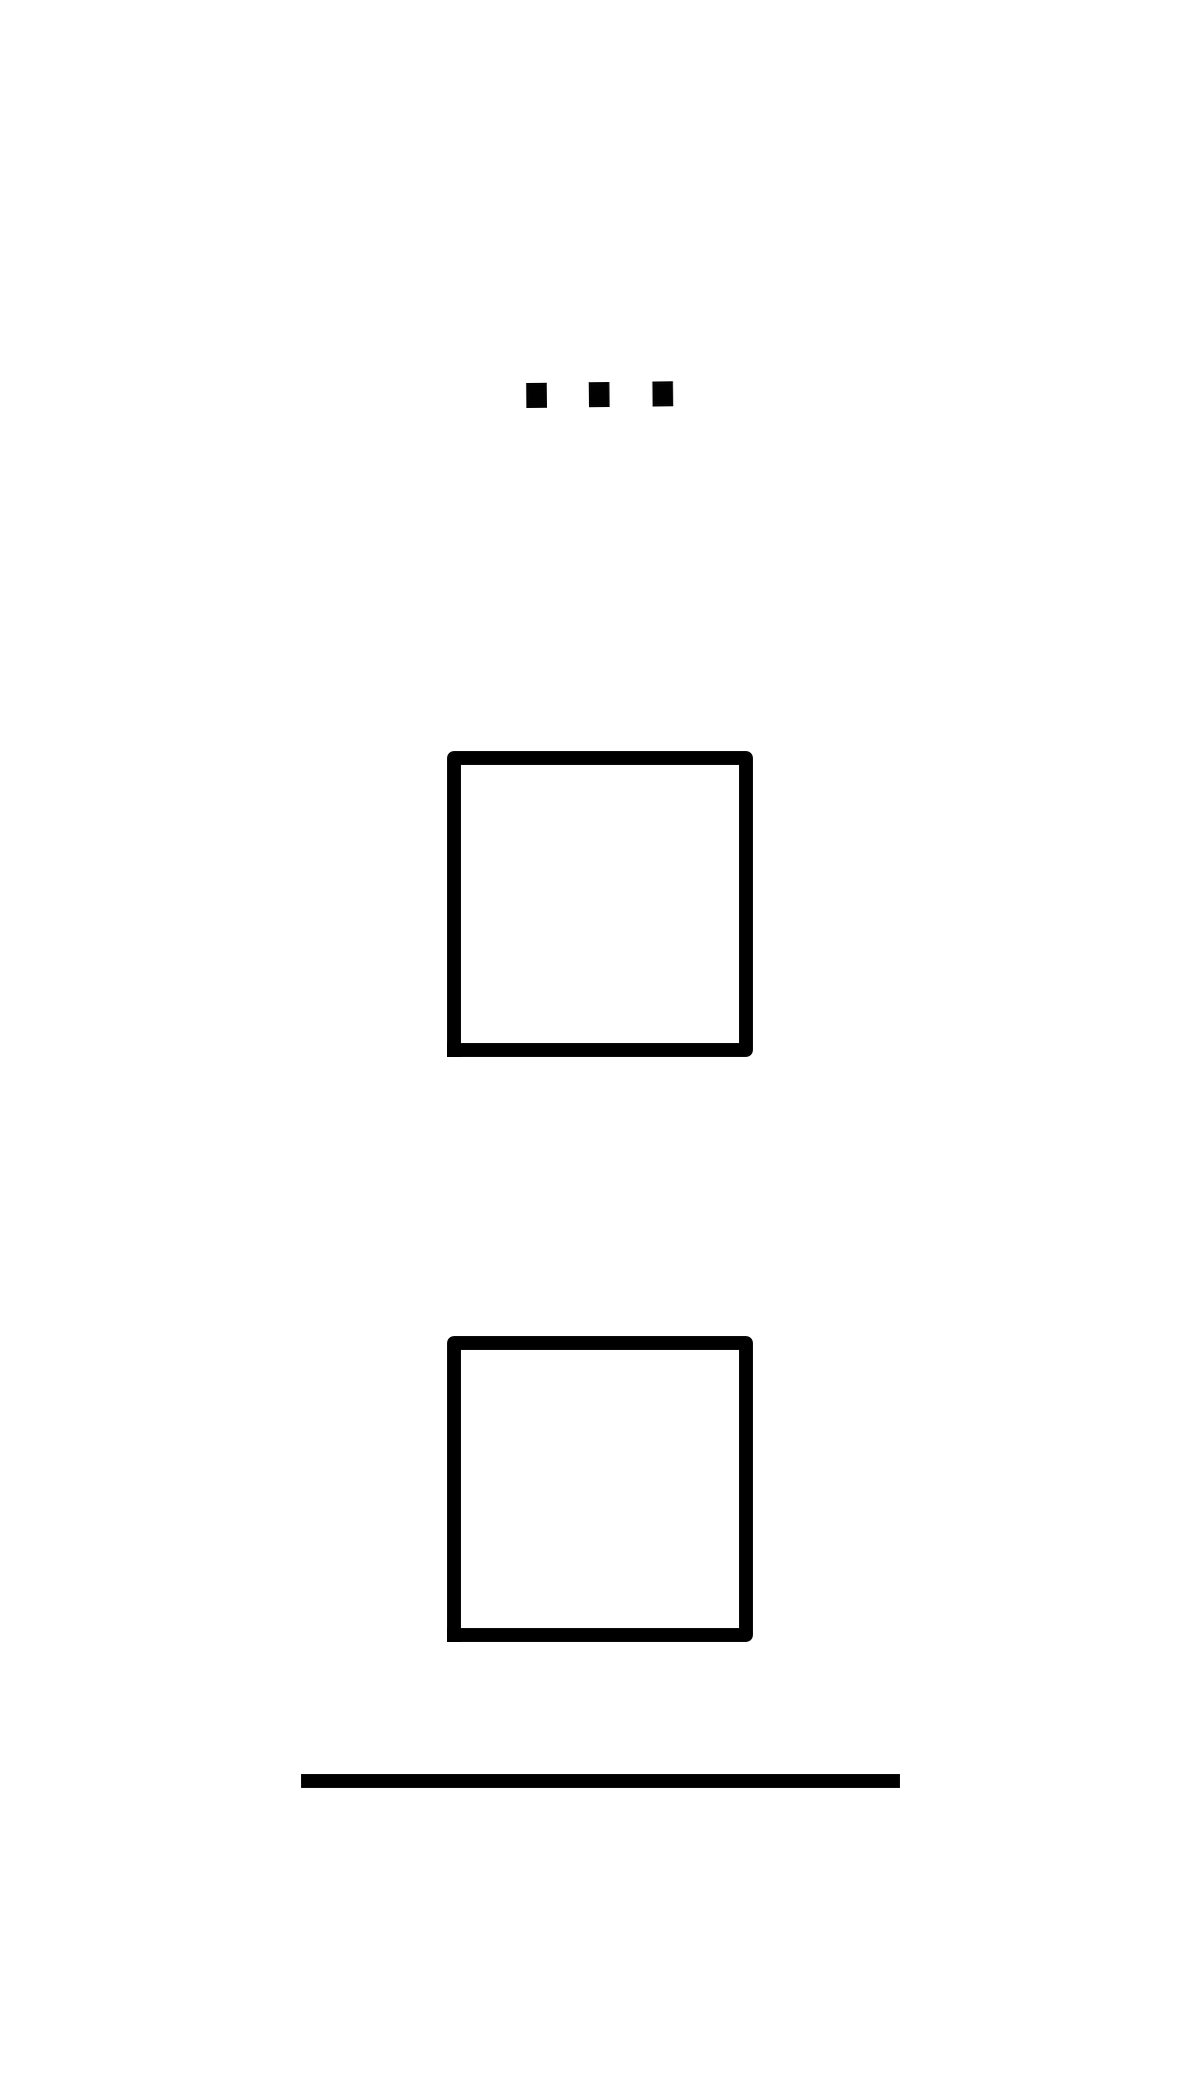
\includegraphics[width=0.3\textwidth]{img4.png}}
\end{center}

The average computational time of a time step is measured and plotted against the number of cubes, $n$.
The average computational time is defined as the average of computational time 
it takes for my machine to simulate the scene in the first $n$ seconds.

\section{Starting Point}

Personally, I have some basic knowledge of programming in C++, having completed a small project using it during my internship.
My graphics knowledge only comes from the two Part IA and IB graphics courses.

Additionally, I have done a bit of research online, 
and am therefore decently confident about the abundance of tutorial resources, 
despite not actually having spent time reading through them.
For example, a full video series about physics engine is available on the Internet\cite{tutorialyt}.
I might also make use of 3D graphics libraries like CUDA\cite{cuda}, but as of now I have no prior working experience with them.

The aforementioned open-source physics engine libraries are also available for me to look into some possible solutions or draw comparisons, 
but I will not be using their simulation code in my project.

\section{Success criteria}

For the core:

\begin{itemize}
\item Implement all basic modules: Object modelling, Collision detection, Bounce, Friction, Stability.

\item Evaluate the engine by comparing it with popular existing engines in the three tests.

\item Demonstrate that the engine works with screenshots of simple examples.
\end{itemize}

For extensions (ordered by priority):

\begin{itemize}
\item Implement fluid dynamics.

\item Implement different versions of the engine for whether GPU is used, and for other interesting parameters like the number of cores used. 
Then draw performance comparisons using the falling test.

\item Implement real-time rendering, which should allow the project to meet all previous criteria without third-party rendering libraries. 

\item Implement soft-body dynamics.
\end{itemize}

\section{Work plan}

\subsection*{Michaelmas term}

\subsubsection*{Now - 15 Oct}

Write project proposal

Research for libraries to use

Environment setup

Milestone: Complete full project proposal

\subsubsection*{16 Oct - 29 Oct}

Set up the project framework

Implement basic interfaces into rendering libraries

Milestone: Able to produce a blank video or an empty interactive demo

\subsubsection*{30 Oct - 19 Nov}

Implement Object Modelling

\subsubsection*{20 Nov - 3 Dec}

Implement Collision Detection

\subsection*{Christmas break}

\subsubsection*{4 Dec - 17 Dec}

Implement Bounce, Friction

\subsubsection*{18 Dec - 14 Jan}

Implement Stability

Milestone: Complete the core

\subsection*{Lent term}

\subsubsection*{15 Jan - 28 Jan}

Buffer phase for core implementation

Core evaluation if core is completed

Write progress report

Milestone: Completed a draft of the progress report

\subsubsection*{29 Jan - 15 Feb}

Buffer phase for core evaluation

Start extension implementations

Finish progress report

Milestone: Submit the Progress Report (Deadline 2 Feb)

\subsubsection*{16 Feb - 1 Mar}

Implement extensions

Start dissertation write up

\subsubsection*{1 Mar - 15 Mar}

Wrap up implementations

Continue writing the dissertation

Milestone: Implementations completed

\subsection*{Easter break}

\subsubsection*{16 Mar - 1 Apr}

Complete a draft of the dissertation, available for view and feedback

Milestone: First draft of dissertation completed

\subsubsection*{2 Apr - 22 Apr}

Improve the dissertation based on the feedback

Milestone: Second draft of dissertation completed

\subsection*{Easter term}

\subsubsection*{23 Apr - 1 May}

Improve the dissertation based on the feedback

Milestone: Third and final draft of dissertation completed

\subsubsection*{2 May - 10 May}

Finalise the dissertation

Milestone: Submit the final dissertation (Deadline 10 May)

\section{Resource declaration}

\begin{itemize}
\item I will be using my personal laptop (specs) as my main working device.
\item For backup and workflow tracking, I will make use of GitHub, Google Drive, and Overleaf
\item For development, I will be using rendering libraries like Blender, as well as GPU interfaces such as CUDA.
\item As a backup plan I have another laptop for working.
\end{itemize}

\bibliographystyle{unsrt}
\bibliography{proposalbib.bib}

\end{document}

\end{document}